\Punto{Definición de derivada}
\begin{ejemplo}
{
    Calcula las siguientes derivadas aplicando la definición:
    \begin{apartados}
     \ap $f(x)=3x^2-2$
     \ap $g(x)=\sqrt{3x+1}$
    \end{apartados}
}
\end{ejemplo}

\Punto{Cálculo de derivadas}
\begin{ejemplo}
{
    Calcula la derivada de las siguientes funciones:
    \begin{apartadosc}
     \ap $\displaystyle{y=2x^3-\frac1x+2^x}$
     \ap $\displaystyle{y=x^3\tan{x}}$
     \ap $\displaystyle{y=\frac{\ln{x}}{2-x}}$
     \ap $\displaystyle{y=(1+\cos{x})^3}$
     \ap $\displaystyle{y=\arctan{(x^3)}}$
     \ap $\displaystyle{y=\frac{2x-1}{(3x+2)^2}}$
    \end{apartadosc}
}
\end{ejemplo}

\Punto{Recta tangente y recta normal}
\begin{ejemplo}{
    Calcula la recta tangente a la curva \[y=\sqrt{e^x+x}\] en el punto de abscisa $x=0$.
}
\end{ejemplo}

\begin{ejemplo}{
    Calcula la recta tangente a la curva \[y=x\ln{x}\] que es perpendicular a la recta $y=-\frac12x+1$.
}
\end{ejemplo}

\Punto{Regla de L'Hôpital}

\begin{ejemplo}{
    Resuelve las siguientes indeterminaciones $\left[\frac00\right]$ y $\left[\frac{\infty}{\infty}\right]$:
    \begin{apartadosc}
        \ap $\displaystyle{
                \lim_{x\to0}\frac{e^x-1}{x}
            }$
        \ap $\displaystyle{
                \lim_{x\to\infty}\frac{\ln{x}}{x^2}
            }$
        \ap $\displaystyle{
                \lim_{x\to0}\frac{x-\tan{x}}{x-\sen{x}}
            }$
    \end{apartadosc}
}
\end{ejemplo}

\begin{ejemplo}{
    Calcula los siguientes límites e indica cuáles presentan una indeterminación:
    \begin{apartadosc}
        \ap $\displaystyle{
                \lim_{x\to0^+}\left(x\cdot\ln{x}\right)
            }$
        \ap $\displaystyle{
                \lim_{x\to\infty}\left[(e^{-x}-1)\cdot x^2\right]
            }$
        \ap $\displaystyle{
                \lim_{x\to0^+}\left(\frac1x-\ln{x}\right)
            }$
        \ap $\displaystyle{
                \lim_{x\to0^+}\left(\ln\sen{x}-\ln\tan{x}\right)
            }$
    \end{apartadosc}
}
\end{ejemplo}

\begin{ejemplo}{
    Calcula los siguientes límites, identificando las indeterminaciones que aparezcan:
    \begin{apartadosc}
        \ap $\displaystyle{
                \lim_{x\to0^+}(1-x)^{2/x}
            }$
        \ap $\displaystyle{
                \lim_{x\to\infty}x^{1/x}
            }$
        \ap $\displaystyle{
                \lim_{x\to0^+}\sin^x{x}
            }$
        \ap $\displaystyle{
                \lim_{x\to\infty}\frac1{x^x}
            }$
    \end{apartadosc}
}
\end{ejemplo}

\Punto{Continuidad y derivabilidad}


\begin{definicion}{Continuidad en un punto.}
Decimos que una función $f(x)$ es continua en un punto $x=c$ si:
\begin{enumerate}
    \item Existe $f(c)$
    \item Existe $\displaystyle{\lim_{x\to c}f(x)}$
    \item El límite y la función coinciden:
        \[f(c)=\lim_{x\to c}f(x)\]
\end{enumerate}
Para que el límite exista los límites laterales tienen que existir y coincidir, así que la condición de continuidad puede expresarse también de la forma:
\[f(c)=\lim_{x\to c^-}f(x)=\lim_{x\to c^+}f(x)\]
\end{definicion}

\begin{definicion}{Continuidad en un intervalo}
\begin{itemize}
    \item Una función es continua en un intervalo abierto $(a,b)$ si es continua en todos los puntos del intervalo.
    \item Una función es continua en un intervalo cerrado $[a,b]$ si es continua en todos los puntos del abierto $(a,b)$ y presenta continuidad lateral en los extremos del intervalo. Es decir:
    \[
        \lim_{x\to a^+}f(x)=f(a)
            \hspace{5mm}\text{y}\hspace{5mm}
        \lim_{x\to b^-}f(x)=f(b)
    \]   
\end{itemize}
\end{definicion}

\begin{definicion}{Clasificación de discontinuidades}
\end{definicion}

\begin{ejemplo}{
    Estudia la continuidad de las siguientes funciones:
    \begin{apartados}
        \ap $\displaystyle{
                f(x)=\frac{e^x-1}{x^2-3x}
            }$
        \ap $\displaystyle{
                f(x)=\frac{\sen{(\pi x)}}{x-\sqrt{x}}
            }$
        \ap $\displaystyle{
                f(x)=\left\{\begin{array}{lcc}
                    \displaystyle{\frac1{x+2}} &\text{si}&x\leqslant0\\
                    \sqrt{x+1}&\text{si}&x>0
                \end{array}\right.
            }$
        \ap $\displaystyle{
                f(x)=\left\{\begin{array}{lcc}
                    \displaystyle{\frac1{x+1}}&\text{si}&x\leqslant0\\
                    \displaystyle{\frac{\tan{(\pi x)}}{\pi x}}&\text{si}&0<x\leqslant\displaystyle{\frac14}\\
                    \displaystyle{\frac{3x+2}{4x-1}}&\text{si}&\displaystyle{\frac14}<x\leqslant3
                \end{array}\right.
            }$
    \end{apartados}
}
\end{ejemplo}

\begin{definicion}{Derivabilidad en un punto.}
Decimos que una función $f(x)$ es derivable en un punto $x=c$ si:
\begin{enumerate}
    \item $f(x)$ es continua en $x=c$.
    \item Existe $f'(c)$ y es finita.
\end{enumerate}
Para que la derivada exista en un punto es necesario que sus derivadas laterales $f'(c^-)$ y $f'(c^+)$ existan, sean finitas y coincidan, es decir:
\[
\begin{aligned}
    f'(c^-)&=\lim_{h\to0^-}\frac{f(c+h)-f(c)}{h}=\\
        &=\lim_{h\to0^+}\frac{f(c+h)-f(c)}{h}=f'(c^+)
\end{aligned}
\]
\end{definicion}

\begin{definicion}{Derivabilidad en un intervalo.}
\begin{itemize}
    \item Una función es derivable en un intervalo abierto $(a,b)$, si es derivable en todos los puntos del intervalo.
    \item Una función es derivable en un cerrado $[a,b]$ si es derivable en el abierto y presenta derivabilidad lateral en los extremos.
\end{itemize}
\end{definicion}

\begin{ejemplo}{
    Estudia la derivabilidad de las siguientes funciones:
    \begin{apartados}
        \ap $\displaystyle{f(x)=x^2\ln{x}}$
        \ap $\displaystyle{f(x)=\sqrt[3]{x+2}}$
        \ap $\displaystyle{
            f(x)=\left\{\begin{array}{lcc}
                x^2&\text{si}&x<1\\
                2x-1&\text{si}&x\geqslant1
            \end{array}\right.
        }$
        \ap $\displaystyle{f(x)=x\cdot|\,e^{x-1}-1\,|}$
    \end{apartados}
}
\end{ejemplo}

\Punto{Teoremas}

\begin{definicion}{Teorema de Bolzano.}
Sea $f(x)$ una función continua en el intervalo cerrado $[a,b]$ tal que $f(a)\cdot f(b)<0$ (la función toma signos opuestos en los extremos del intervalo), entonces:
\[\exists c\in(a,b)\mid f(c)=0\]
$$\begin{tikzpicture}
\begin{axis}[
    yscale=0.6,
    axis lines=middle,
    xlabel={$x$},
    ylabel={$y$},
    xtick=\empty,
    ytick=\empty,
    xmin=-0.5, xmax=3.5,
    ymin=-1.3, ymax=2,
]
    \node at (0.5,0) [below] {$a$};
    \node at (3,0)   [above] {$b$};
    \node at (1.75,0) [below] {$c$};
    \draw[dotted] (0,1) node[left] {$f(a)$} -- (0.5,1) -- (0.5,0);
    \draw[dotted] (0,-1) node[left] {$f(b)$} -- (3,-1) -- (3,0);
    \draw[thick] (0.5,1) .. controls (1.5,1.5) and (1.5,-0.5) .. 
                 (3,-1);
    \fill (0.5,1) ellipse (0.03 and 0.05);
    \fill (3,-1) ellipse (0.03 and 0.05);
\end{axis}
\end{tikzpicture}$$
\end{definicion}

\begin{ejemplo}{
Comprueba que la función $f(x)=x^3+5x-13$ tiene solución real y acota una de sus soluciones con un error menor a $\dfrac14$.}
\end{ejemplo}

\begin{ejemplo}{
Comprueba que la función:
\[f(x)=\left\{\begin{array}{lcc}
    \displaystyle{\frac{1-e^x}{x}}&\text{si}&x<0\\
    x+e^x-2&\text{si}&x\geqslant0
\end{array}\right.
\]
cumple las condiciones para aplicar el teorema de Bolzano en el intervalo $[-2,2]$. Acota una posible solución entre dos números enteros consecutivos.
}
\end{ejemplo}

\begin{ejemplo}{
Demuestra que las gráficas de las funciones:
\[
    f(x)=e^x
    \hspace{5mm}\text{y}\hspace{5mm}
    g(x)=\frac1{x+5}
\]
Se cortan en al menos un punto, acota la abscisa de su punto de corte entre dos enteros consecutivos.}
\end{ejemplo}

\begin{definicion}{Teorema de Rolle.}
Dada una función $f(x)$ continua en el intervalo $[a,b]$ y derivable en el intervalo $(a,b)$, tal que $f(a)=f(b)$, se cumple:
\[\exists c\in(a,b)\mid f'(c)=0\]
$$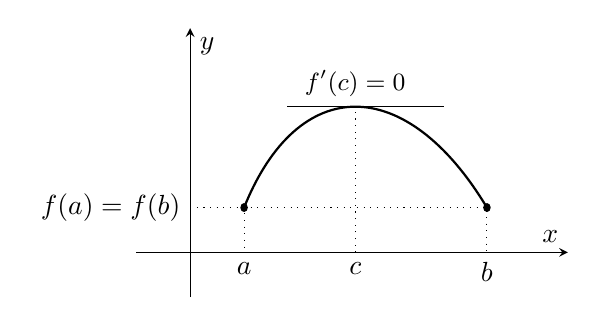
\begin{tikzpicture}
\begin{axis}[
    yscale=0.6,
    axis lines=middle,
    xlabel={$x$},
    ylabel={$y$},
    xtick=\empty,
    ytick=\empty,
    xmin=-1.5, xmax=3.5,
    ymin=-0.5, ymax=2.5,
]
    \node at (0.5,0)  [below] {$a$};
    \node at (2.75,0) [below] {$b$};
    \draw[dotted] (1.53,0) node[below] {$c$} -- 
                  (1.53,1.63) node[above] {\small $f'(c)=0$};
    \draw[thin] (0.9,1.63) -- (2.35,1.63);
    \draw[dotted] (0,0.5) node[left] {$f(a)=f(b)$} -- 
                  (0.5,0.5) -- 
                  (0.5,0);
    \draw[dotted] (0.5,0.5) -- (2.75,0.5) -- (2.75,0);
    \draw[thick] (0.5,0.5) .. controls (1,2) and (2,2) .. 
                 (2.75,0.5);
    \fill (0.5,0.5)  ellipse (0.035 and 0.05);
    \fill (2.75,0.5) ellipse (0.035 and 0.05);
    \draw[very thick,white] (-2,0) -- (-0.5,0);
\end{axis}
\end{tikzpicture}$$
\end{definicion}

\begin{ejemplo}{
    Demuestra que la función:
    \[f(x)=x\ln{(x+2)}\]
    tiene, al menos un punto en el intervalo $(-1,0)$ tal que $f'(x)=0$
}
\end{ejemplo}

\begin{ejemplo}{
    Dada la función:
        \[f(x)=2x+\sen{x}\]
    Demuestra que existe un único punto $c$ tal que $f(c)=2$
}
\end{ejemplo}

\begin{definicion}{Teorema del valor medio de Lagrange.}
Dada una función $f(x)$ continua en el intervalo $[a,b]$ y derivable en el intervalo $(a,b)$, se cumple:
\[\exists c\in(a,b)\mid f'(c)=\frac{f(b)-f(a)}{b-a}\]
$$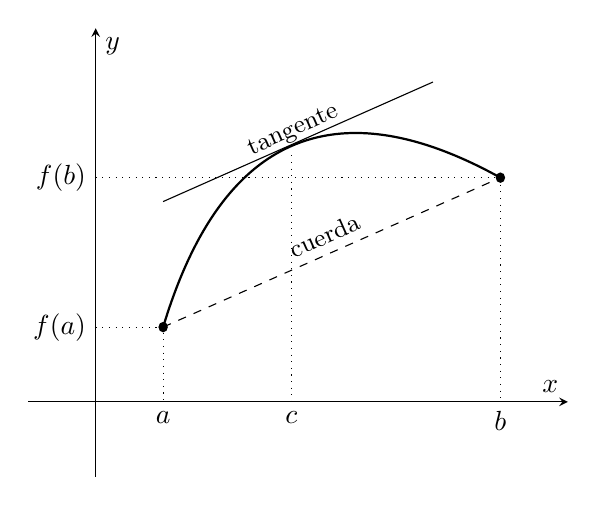
\begin{tikzpicture}
\begin{axis}[
    axis lines=middle,
    xlabel={$x$},
    ylabel={$y$},
    xtick=\empty,
    ytick=\empty,
    xmin=-0.5, xmax=3.5,
    ymin=-0.5, ymax=2.5,
]
    \node at (0.5,0) [below] {$a$};
    \node at (3,0)   [below] {$b$};
    \draw[dotted] (1.45,1.65) -- (1.45,0) node[below] {$c$};
    \draw[dotted] (0,0.5) node[left] {$f(a)$} -- 
                  (0.5,0.5) -- 
                  (0.5,0);
    \draw[dotted] (0,1.5)  node[left] {$f(b)$}-- 
                  (3,1.5) -- 
                  (3,0);
    \draw[thick] (0.5,0.5) .. controls (1,2) and (2,2) .. 
                 (3,1.5);
    \draw[dashed] (0.5,0.5) -- 
                  (3,1.5) node[above,midway,sloped] {\small cuerda};
    \draw (0.5,1.34) -- (2.5,2.14) node[above=-1mm,midway,sloped] {\small tangente};
    \fill (0.5,0.5)  ellipse (0.035 and 0.035);
    \fill (3,1.5) ellipse (0.035 and 0.035);
    %\draw[very thick,white] (-2,0) -- (-0.5,0);
\end{axis}
\end{tikzpicture}$$
\end{definicion}

\begin{ejemplo}{
Dada la función:
    \[f(x)=x^3+2\]
Demuestra que existe algún punto en el intervalo $(-1,1)$, tal que la función $f'(x)=1$. Calcula el valor, o valores en que esto ocurre.
}
\end{ejemplo}

\Punto{Asíntotas}
\begin{definicion}{Asíntotas verticales (AV).}
La recta $x=c$ es una asíntota vertical de una función si alguno de sus límites laterales en $c$ es $+\infty$ o $-\infty$.
\begin{itemize}
    \item Una función puede tener cualquier número de asíntotas verticales.
    \item La función puede estar definida en $c$ aunque tenga una asíntota vertical allí; asignar un valor aislado $f(c)$ no modifica los límites laterales.
\end{itemize}
\end{definicion}

\begin{definicion}{Asíntotas horizontales (AH).}
Una función tiene una asíntota horizontal de ecuación $y=c$ si:
$$\lim_{x\to+\infty}f(x)=c\hspace{5mm}\text{o}\hspace{5mm}\lim_{x\to-\infty}f(x)=c$$
\begin{itemize}
    \item Una función puede tener, a lo sumo, dos asíntotas horizontales, una hacia $+\infty$ y otra hacia $-\infty$.
    \item Si la función es racional $f(x)=\frac{P(x)}{Q(x)}$ y tiene asíntota horizontal, esta es única y coincide con el cociente de la división entre polinomios.
    \item Una función puede cortar a sus asíntotas horizontales.
\end{itemize}
\end{definicion}

\begin{definicion}{Asíntotas oblicuas (AO).}
Una función tiene una asíntota oblicua $y=mx+n$, con $m\ne0$, si
$$\exists m,\,n\in\mathbb{R}\mid m=\lim_{x\to+\infty}\frac{f(x)}{x}\hspace{3mm}\text{y}\hspace{3mm}n=\lim_{x\to+\infty}\left[f(x)-mx\right]$$
\hfil o \hfil
$$\exists m,\,n\in\mathbb{R}\mid m=\lim_{x\to-\infty}\frac{f(x)}{x}\hspace{3mm}\text{y}\hspace{3mm}n=\lim_{x\to-\infty}\left[f(x)-mx\right]$$
\begin{itemize}
    \item Una función puede tener, a lo sumo, dos asíntotas oblicuas, una hacia $+\infty$ y otra hacia $-\infty$.
    \item Si la función es racional $f(x)=\frac{P(x)}{Q(x)}$ y tiene asíntota oblicua, esta es única y coincide con el cociente de la división entre polinomios.
    \item Una función puede cortar a sus asíntotas oblicuas.
\end{itemize}
\end{definicion}

\begin{ejemplo}{
Encuentra las asíntotas de las siguientes funciones y represéntalas:
\begin{apartados}
    \ap $f(x)=\dfrac{x^3+2x}{5}$
    \ap $f(x)=\dfrac{x^3-2x}{2x^2+3x}$
    \ap $f(x)=\left\{\begin{array}{lcc}
            \dfrac{x^2}{x-1}&\text{si}&x\leqslant0\\
            \dfrac{\ln{x}}{x}&\text{si}&x>0
        \end{array}\right.$
    \ap $f(x)=\sqrt{2x^2+1}$
    \ap $f(x)=\dfrac{e^x}{e^x+1}$
\end{apartados}
}
\end{ejemplo}

\Punto{Monotonía}
\begin{definicion}{Monotonía.}
Una función $f(x)$, derivable en el intervalo $(a,b)$, es monótonamente creciente en dicho intervalo si: 
    $$f'(x)>0\mid x\in(a,b)$$
Una función $f(x)$, derivable en el intervalo $(a,b)$, es monótonamente decreciente en dicho intervalo si: 
    $$f'(x)<0\mid x\in(a,b)$$
\end{definicion}

\begin{definicion}{Extremos relativos.}
Una función tiene un máximo relativo en $x=c$ si $f(c)\geqslant f(x)$ para todos los puntos de su dominio suficientemente próximos a $c$. Tiene un mínimo relativo si $f(c)\leqslant f(x)$ en ese entorno.

Si la función es derivable en $c$ y tiene allí un extremo relativo interior, necesariamente $f'(c)=0$. Esta condición por sí sola no garantiza la existencia de un extremo.

Si la función es continua en $c$, un cambio de monotonía permite distinguir:
\begin{itemize}
    \item \textbf{Máximo relativo}: la función pasa de creciente a decreciente.
    \item \textbf{Mínimo relativo}: la función pasa de decreciente a creciente.
\end{itemize}
También puede haber extremos relativos en puntos donde la función no sea derivable.
\end{definicion}

\begin{definicion}{Extremos absolutos}
Una función tiene un \textbf{máximo absoluto} en $x=c$ si $f(c)\geqslant f(x)$ para todo $x$ de su dominio. Tiene un \textbf{mínimo absoluto} si $f(c)\leqslant f(x)$ para todo $x$ de su dominio.

La menor cota superior se llama \textbf{supremo}. Si se alcanza, es el máximo absoluto; si no se alcanza, la función no tiene máximo absoluto.

La mayor cota inferior se llama \textbf{ínfimo}. Si se alcanza, es el mínimo absoluto; si no se alcanza, la función no tiene mínimo absoluto.
\end{definicion}

\begin{ejemplo}{
Estudia el crecimiento y los extremos de las siguientes funciones:
\begin{apartados}
 \ap $\displaystyle{f(x)=x^4-x^2}$
 \ap $\displaystyle{f(x)=\frac{x^3}{(x-1)^2}}$
 \ap $\displaystyle{f(x)=\sqrt[3]{(x+1)^2}}$
 \ap $\displaystyle{f(x)=\left\{\begin{array}{lcc}
        e^{x-1}&\text{si}&x<1\\
        (x-2)^2&\text{si}&x\geqslant1
    \end{array}\right.}$
\end{apartados}
}
\end{ejemplo}

\begin{ejemplo}{
Representa las siguientes funciones basándote en sus asíntotas y en su monotonía:
\begin{apartados}
    \ap $\displaystyle{f(x)=\sqrt{|x|+\frac1{|x|}}}$
    \ap $\displaystyle{f(x)=\frac{x^3}{(x+1)^2}}$
    \ap $\displaystyle{f(x)=\ln^2{x}}$
\end{apartados}
}
\end{ejemplo}

\begin{ejemplo}{
En cierto ecosistema, la población de cierta especie después de una enfermedad que reduce significativamente su número de depredadores se puede modelar por la función:
\[P(t)=\frac{4e^{t/2}-t^2-2}{e^{t/2}}\]
donde $t$ se refiere al tiempo en años medido desde el instante en que los depredadores perecen y $P$ a la población en miles de individuos.
\begin{apartados}
    \ap ¿Cuál es la población inicial de la especie?
    \ap La población descontrolada de la especie produce una escasez de comida que con el tiempo produce una mortandad, ¿en qué momento se alcanza la mínima población de la especie?
    \ap ¿Cuál es la evolución de la población a largo plazo?
\end{apartados}
}
\end{ejemplo}

\begin{ejemplo}{
Tomamos un punto $P$ de la función $f(x)=1-x^2$ con\\ $0\leqslant x\leqslant1$ y proyectamos dicho punto sobre los ejes de coordenadas obteniendo los puntos $Q$ y $R$. ¿Cuáles deben ser las coordenadas de $P$ para que el rectángulo $OQPR$ tenga área máxima?
}
\end{ejemplo}

\begin{ejemplo}{
Tomamos una cartulina en forma de sector circular de radio $R=1$ y longitud de arco $L$ y construimos un cono uniendo los dos radios del sector. ¿Para qué valor de $L$ obtendremos un cono de volumen máximo?
}
\end{ejemplo}

\begin{ejemplo}{
Un aldeano situado en el punto $P(0,1)$ quiere llenar una garrafa de agua en un río cuya orilla más cercana coincide con la recta $y=0$ y llevarla a su pueblo situado en el punto $Q(3,2)$. Si pretende recorrer el mínimo camino posible, ¿en qué punto deberá llenar la garrafa?
}
\end{ejemplo}

\Punto{Métodos de Integración}
\begin{ejemplo}{
Calcula las siguientes integrales de funciones racionales:
\begin{apartados}
 \ap $\displaystyle{\int\frac{x^3+2x-1}{x+2}\,dx}$
 \ap $\displaystyle{\int\frac{6x+5}{2x^2+5x-3}\,dx}$
 \ap $\displaystyle{\int\frac{2x-1}{x^2+4x+4}\,dx}$
 \ap $\displaystyle{\int\frac{x^3-1}{x^2+x}\,dx}$
 \ap $\displaystyle{\int\frac{x}{x^2+x+2}\,dx}$
\end{apartados}
}
\end{ejemplo}

\begin{ejemplo}{Resuelve las siguientes integrales mediante integración por partes:
\begin{apartados}
    \ap $\displaystyle{\int (3x+1)e^{2x}\,dx}$
    \ap $\displaystyle{\int x^2\cos{x}\,dx}$
    \ap $\displaystyle{\int\arcsen{x}\,dx}$
    \ap $\displaystyle{\int 2x\ln{(x^2-1)}\,dx}$
\end{apartados}
}
\end{ejemplo}

\begin{ejemplo}{
Resuelve las siguientes integrales mediante cambio de variable. Se indican el cambio sugerido y la integral transformada:
\begin{apartados}
    \ap $\displaystyle\int\ln^2 x\,dx$, con $t=\ln x$:
        $\displaystyle\int t^2e^t\,dt$.
    \ap $\displaystyle\int\tan^3 x\,dx$, con $t=\tan x$:
        $\displaystyle\int\dfrac{t^3}{1+t^2}\,dt$.
    \ap $\displaystyle\int\dfrac{\sqrt{x}}{1+x}\,dx$, con $t=\sqrt{x}$:
        $\displaystyle\int\dfrac{2t^2}{1+t^2}\,dt$.
    \ap $\displaystyle\int\dfrac1{e^x+1}\,dx$, con $t=e^x$:
        $\displaystyle\int\dfrac1{t(t+1)}\,dt$.
\end{apartados}
}
\end{ejemplo}

\Punto{Integral definida}

\begin{ejemplo}{
Calcula las siguientes integrales definidas:
\begin{apartados}
 \ap $\displaystyle{\int_0^{\,2}(x^2-x)\,dx}$
 \ap $\displaystyle{\int_{-1}^{\,1}\tan{x}\,dx}$
 \ap $\displaystyle{\int_e^{\,e^2}\sqrt{x}\ln{x}\,dx}$
\end{apartados}
}
\end{ejemplo}

\begin{ejemplo}{
    Calcula el área encerrada entre la curva $y=x^2-2x$ y el eje $OX$ en el intervalo $[-1,1]$.
}
\end{ejemplo}

\begin{ejemplo}{
    Calcula el área encerrada por la función $y=\sqrt{1-x}$ y los ejes de coordenadas.
}
\end{ejemplo}

\begin{ejemplo}{
    Calcula el área encerrada por las curvas $y=x^3+x^2$ e $y=x^2+x$.
}
\end{ejemplo}

\begin{ejemplo}{
    Calcula el área encerrada por la función $f(x)=\ln{x}$, la recta $y=\dfrac{x}e\,$ y el eje de abscisas.
}
\end{ejemplo}

\begin{ejemplo}{
    Calcula el volumen generado por la rotación de la curva $y=x^2+1$ alrededor del eje $OX$ en el intervalo $[0,1]$.
}
\end{ejemplo}

\begin{ejemplo}{
    Calcula el volumen generado cuando la región determinada por las funciones $y=x$ e $y=x^2$ gira alrededor del eje $OX$.
}
\end{ejemplo}
